\documentclass[10pt,letterpaper]{article} 
\usepackage{tikz}
\usepackage{toolsper}
%\usepackage{graphicx}‎‎
%\usefonttheme{serif}‎
%\usepackage{ptext}‎
%\usepackage{xepersian}
%\settextfont{B Nazanin}
\usepackage{lipsum}
\setlength{\parindent}{0pt}
%\usepackage{enumitem}
%\setlist[enumerate,1]{label=(\arabic*)}
\newcommand{\pf}{$\blacksquare$}
\newcommand{\EX}{\Bbb E}
\newcommand{\nl}{\newline\newline}

\usepackage{amsmath}
\usepackage{accents}
\newlength{\dhatheight}
\newcommand{\doublehat}[1]{%
    \settoheight{\dhatheight}{\ensuremath{\hat{#1}}}%
    \addtolength{\dhatheight}{-0.35ex}%
    \hat{\vphantom{\rule{1pt}{\dhatheight}}%
    \smash{\hat{#1}}}}

\newcounter{QuestionNumber}
\setcounter{QuestionNumber}{1}

\newcommand{\Q}{
\textbf{
سوال \theQuestionNumber)
}
\stepcounter{QuestionNumber}
}

\newcommand{\fig}[3]{
\begin{figure}[h!]
#1
\caption{#2}
\label{#3}
\end{figure}
}

\newcommand{\subfig}[3]{
\begin{subfigure}{#3}
#1
\caption{#2}
\end{subfigure}
}

\newcommand{\figno}[1]{
\begin{figure}[h!]
#1
\end{figure}
}

\newcommand{\subfigno}[2]{
\begin{subfigure}{#2}
#1
\end{subfigure}
}
%\newcommand{\pic}[2]{
%\begin{center}
%\includegraphics[width=#2]{#1}
%\end{center}
%}
\begin{document}
\Large
\begin{center}
به نام زیبایی

یک سوال از نمونه برداری
\hl
\end{center}
الف) اگر نمونه برداری را روی هر دو سیگنال پیوسته اعمال کنیم، طیف سیگنال ها به شکل زیر خواهند بود:
\begin{figure}[h!]
\centering
%%%%%%%%%
\begin{subfigure}{0.49\textwidth}
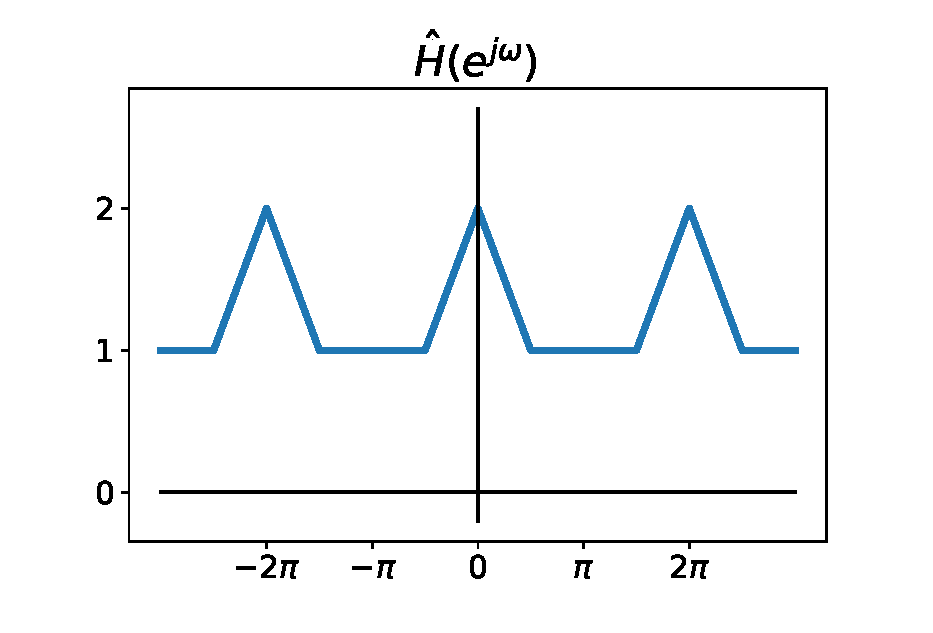
\includegraphics[width=80mm]{SQ_1.eps}
\end{subfigure}
%%%%%%%%%
\begin{subfigure}{0.49\textwidth}
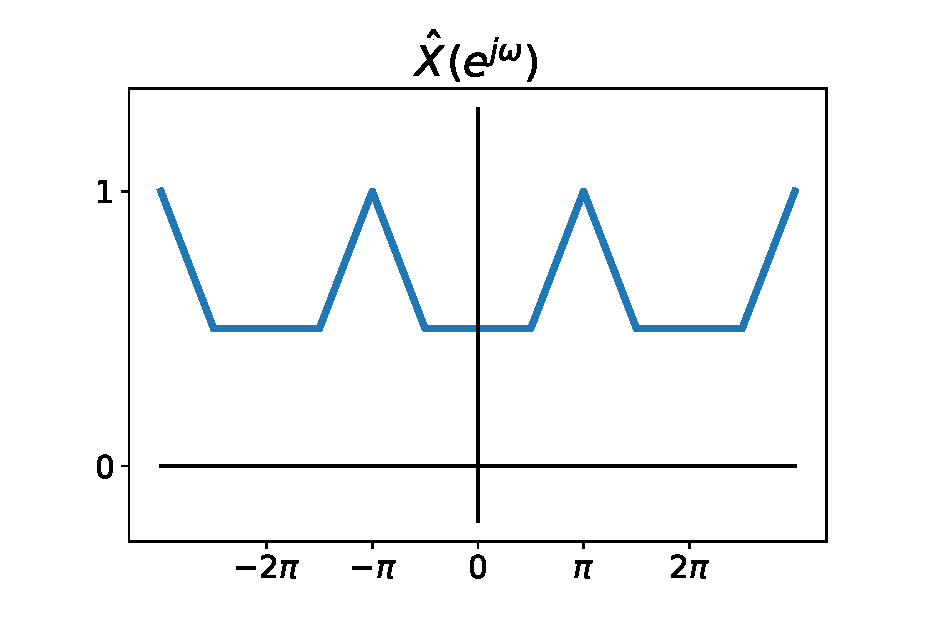
\includegraphics[width=80mm]{SQ_2.eps}
\end{subfigure}
%%%%%%%%%
\end{figure}

ب) اگر تبدیل فوریه های 
$
\hat x[n]
$
 و
$
\hat h[n]
$
 را در هم ضرب کرده، تبدیل 
$
\hat y[n]
$
را یافته و سپس معادل زمان پیوسته آن را بیابیم، خواهیم داشت:
\begin{figure}[h!]
\centering
%%%%%%%%%
\begin{subfigure}{0.49\textwidth}
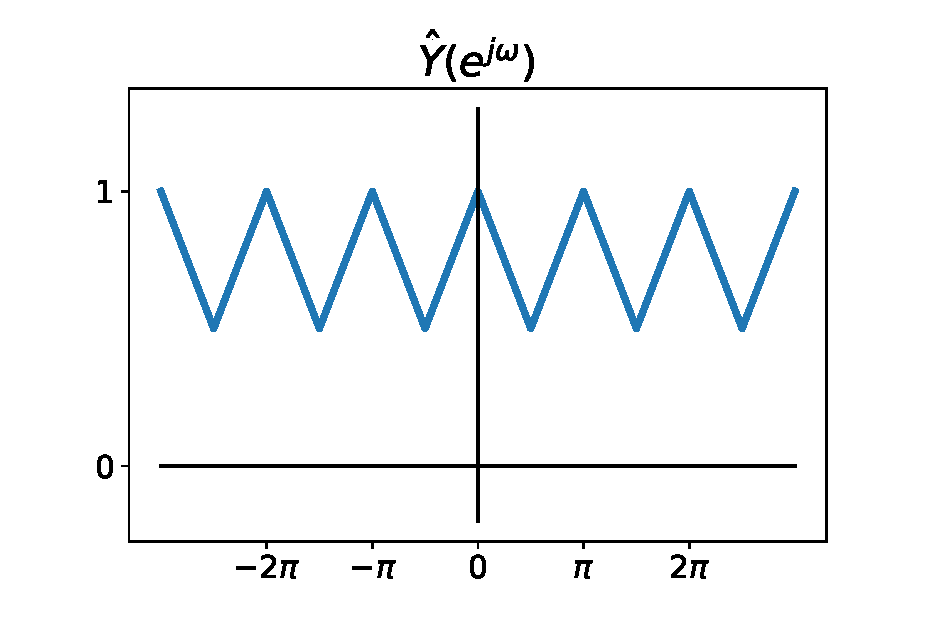
\includegraphics[width=80mm]{SQ_3.eps}
\end{subfigure}
%%%%%%%%%
\begin{subfigure}{0.49\textwidth}
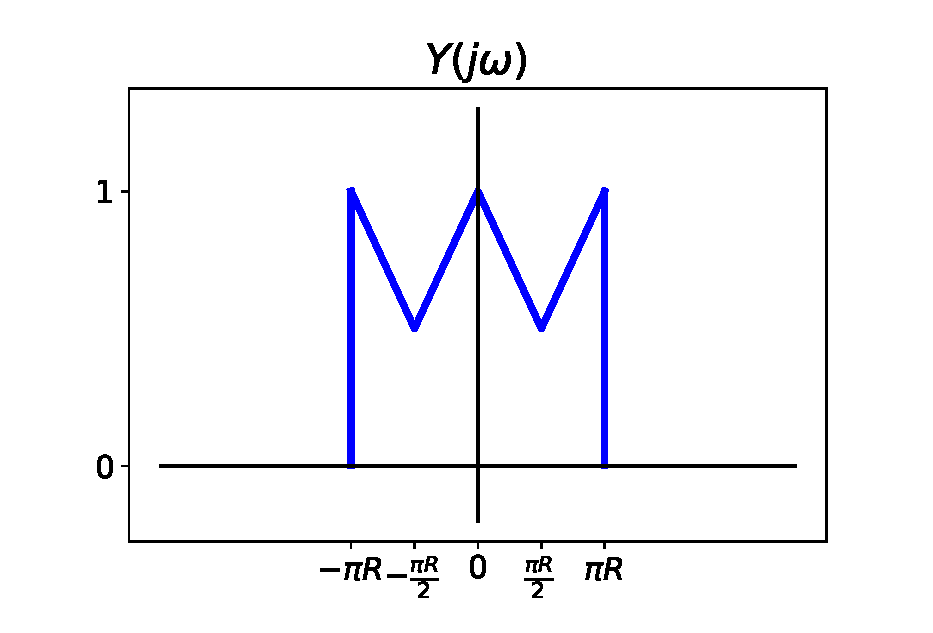
\includegraphics[width=80mm]{SQ_4.eps}
\end{subfigure}
%%%%%%%%%
\end{figure}

پ) براحتی می توان دید که اگر سیگنال 
$
y_c(t)
$
 را به صورت 
$
y_c(t)=x(t)*h(t)
$
تعریف کنیم، رابطه‌ی 
$
Y_c(j\omega)=X(j\omega)H(j\omega)
$
نتیجه می شود. بنابراین با تعریف فوق:
$$
\hat Y_c(e^{j\omega})=\hat X(e^{j\omega})\hat H(e^{j\omega})\implies \hat Y_c(e^{j\omega})=\hat Y(e^{j\omega})\implies Y_c(j\omega)=Y(\omega)
$$
از آنجا که aliasing رخ نمی دهد، می توان گفت نتیجه گیری فوق همواره برقرار است و می توان نوشت:
$$
\hat y[n]=y_c({n\over R_s})
$$

ت) اگر فقط یکی از 
$
x(t)
$
 یا 
$
h(t)
$
 باند محدود باشند، می توان گفت که خروجی که از حاصلضرب تبدیل فوریه‌ی این دو سیگنال به دست می آید نیز باند محدود است (زیرا مقادیر صفر فرکانسی یک سیگنال، مقادیر غیرصفر فرکانسی سیگنال دیگر را صفر می کند)؛ به همین علت پاسخ مثبت است. 
\end{document}